%{{{ Heading Stuff

%{{{ Documentclass, usepackages
%\documentclass[ngerman, landscape]{scrartcl}
\documentclass[ngerman]{scrartcl}
\usepackage[ngerman]{babel}
\usepackage{graphicx}
%}}}

%{{{ Titel, Author, etc...

\newcommand{\blattnummer}{10}												%% Nummer des Übungsblattes angeben
\newcommand{\aufgabe}{1}
\newcommand{\myauthor}{Moritz Nöltner, Johannes Visintini, Philip Bell}
\newcommand{\mytutor}{Amin Kiem}
\newcommand{\mytitle}{Abgabe für ISW Blatt \blattnummer}
\title{\mytitle}
\author{\myauthor}
%}}}

%{{{ Kopf und Fußzeilen einrichten
\usepackage{fontspec, fancyhdr}
\pagestyle{fancy}

\lhead{\bfseries \mytitle}
%%\chead{\mytitle}
\rhead{\bfseries \myauthor}

\lfoot{\bfseries \today}
\cfoot{Tutor: \mytutor}
\rfoot{\bfseries \thepage}

\renewcommand{\headrulewidth}{1pt}
\renewcommand{\footrulewidth}{1pt}
%\textheight = 592pt	%% Standardwert
\textheight = 650pt 	%% Für Hochformat
%%\textheight = 450pt 	%% Für Querformat
%}}}

%{{{ Longtable

\usepackage{multirow}
\usepackage{array}
\usepackage{longtable}
\usepackage{pdfpages}
%}}}

%{{{ Minted (Highlighter für Code)

%% \usepackage{minted}
%% \definecolor{bg}{rgb}{0.95,0.95,0.95}
%% \newminted[Java]{java}{numbersep=5pt, bgcolor=bg, gobble=0, linenos, tabsize=4}
%}}}


%}}}

\begin{document}
	\setcounter{section}{\blattnummer}
	\setcounter{subsection}{\aufgabe-1}
	\subsection{Metriken zum MovieManager}

	\subsubsection*{\underline{Metriken}}
	\begin{figure}[h]
		\centering
		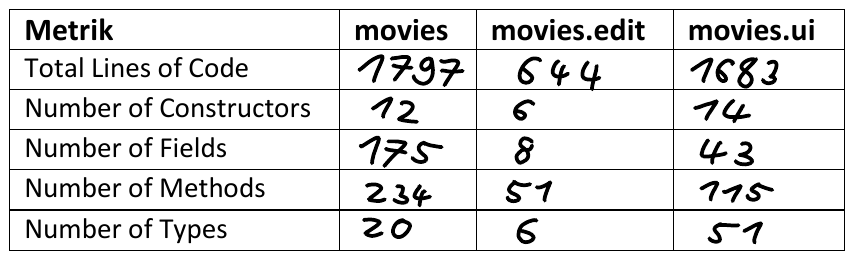
\includegraphics[width=\linewidth]{a101.png}
	\end{figure}

	\subsubsection*{\underline{Vergleiche}}
	\begin{description}
	\item[Total Lines of Code]
		Offensichtlich sind \emph{movies} und \emph{movies.ui} deutlich größer als \emph{movies.edit}. Dies liegt wahrscheinlich daran, dass ihr Funktionsumfang größer ist. Immerhin kapselt das eine die Filme, während das Andere die GUI aufbaut.

	\item[Number of Constructors]
		Eigentlich eine relativ unspektakulärer Vergleich: In Relation zur Anzahl der Quelltextzeilen haben alle Drei gleich viele Konstruktoren.

	\item[Number of Fields]
		Hier setzt sich \emph{movies} deutlich von den Andren ab, da es die eigentlich zu verwaltenden Daten kapselt. Da \emph{movies.edit} eigentlich größtenteils Funktionalität bereit stellt (und deutlich kleiner ist, als der Rest), hat es am wenigsten Felder, während in \emph{movies.ui} noch einige Felder für die GUI-Elemente anfallen.


	\item[Number of Methods]
		Auch hier liegt \emph{movies} deutlich vor den Anderen. Dies dürfte zum größten Teil Settern und Gettern für die vielen Attribute geschuldet sein. Bei \emph{movies.ui} fallen die Attribute hier nicht so sehr ins Gewicht, weil die meisten GUI-Elemente nicht nach außen weitergereicht werden, oder entsprechende Funktionen schon von der Elternklasse ererbt wurden.

	\item[Number of Types]
		Da \emph{movies.ui} viele Klassen enthält, die von GUI-Klassen erben, implementiert es viele Typen, \emph{movies.edit} implementiert keine Interfaces und erbt nicht, da es einen mehr oder minder einmaligen Bedarf deckt, und hat daher nur einen Typ mehr, als es Klassen gibt.
	\end{description}


\end{document}
